\documentclass[11pt]{article}
%Gummi|061|=)
\usepackage{amsmath}
\usepackage{amsthm}
\usepackage{amsbsy}
\usepackage{amssymb}
\usepackage{inputenc}
\usepackage{graphicx}
\usepackage{selinput}
\usepackage{here}
\SelectInputMappings{%
adieresis={ä},
germandbls={ß},
}
\title{\textbf{Versuch V204: Wärmeleitung von Metallen}}
\author{Martin Bieker\\
		Julian Surmann\\
		\\
		Durchgef\"{u}hrt am 31.10.2013\\
		Tu Dortmund}
\date{}
\usepackage{graphicx}
\begin{document}
\renewcommand\tablename{Tabelle}
\renewcommand\figurename{Abbildung}
\maketitle
\thispagestyle{empty}
\newpage
\clearpage
\setcounter{page}{1}


\section{Einleitung}
Im folgenden Versuch geht es um die Untersuchung von Wärmeleitung. Unter Wärmeleitung versteht man den Fluss von Wärme in Richtung geringerer Temparatur. Es wird die Wärmeleitung von mehreren Metallen untersucht. 
\section{Theorie}
Für die Untersuchung des Wärmetransportes in Metallen wird hier nur die Wärmeleitung betrachtet, Konvektion und Wärmestrahlung sind vernachlässigbar.
Die Wärmemenge, die in einer Zeit dt durch die Querschnittsfläche A des zu untersuchenden Stabes fließt, ist gegeben durch:
\begin{equation}
dQ = -\kappa A \frac{\partial T}{\partial x} dt.
\end{equation}
Die Wärmestromdichte $j_w$ ist dann gegeben mit
\begin{equation}
j_w = -\kappa \frac{\partial T}{\partial x}.
\end{equation}
Aus Formel (2) und der Kontinuitätsbedingung lässt sich eine eindimensionale Wärmeleitungsgleichung herleiten:
\begin{equation}
\frac{\partial T}{\partial t} = \frac{\kappa}{\rho c} \frac{\partial^2 T}{\partial x^2}.
\end{equation}
Diese Gleichung gibt die zeitliche und räumliche Entwicklung der Temparaturverteilung an. $c$ steht hier für die spezifische Wärme des Metalles, $\rho$ für dessen Dichte.
$\sigma_T = \frac{\kappa}{\rho c}$ steht damit für die Temparaturleitfähigkeit des Materials. Die Temparaturleitfähigkeit ist ein Maß für Geschwindigkeit, mit der Temparaturdifferenzen neutralisiert werden.
Im zweiten Versuchsteil soll das Ende verschiedener Metallstäbe periodisch erwärmt und gekühlt werden. Dabei entsteht eine räumliche und zeitliche Temparaturwelle. Diese hat die Form
\begin{equation}
T(x,t) = T_{max} e^{\sqrt{\frac{w \rho c}{2 \kappa}}x}cos \left( wt- \sqrt{\frac{w \rho c}{2 \kappa}}x \right).
\end{equation}
Die Phasengeschwindigkeit der Welle ist gegeben mit
\begin{equation}
v = \frac{w}{k} = \frac{w}{\sqrt{\frac{w \rho c}{2 \kappa}}} = \sqrt{\frac{2 \kappa w}{\rho c}}
\end{equation}
Mithilfe der Dämpfung, die aus dem Verhältnis $\frac{A_{nah}}{A_{fern}}$ folgt, und der Ausdrücke $w = \frac{2 \pi}{T^*}$ ($T^*$ steht für die Periodendauer, nicht für eine Temparatur) und $\Phi = 2 \pi \frac{\Delta t}{T^*}$ folgt für die Wärmeleitfähigkeit
\begin{equation}
\label{kappa}
\kappa = \frac{\rho c (\Delta x)^2}{2 \Delta t ln(\frac{A_{nah}}{A_{fern}})}
\end{equation}
Hierbei beschreibt $\Delta x$ den Abstand zwischen den beiden Temparaturmessstellen und $\Delta t$ die Phasendifferenz der Wärmewelle zwischen den beiden Messstellen.
\section{Aufbau und Durchf\"{u}hrung}
\begin{figure}[htp]
\centering
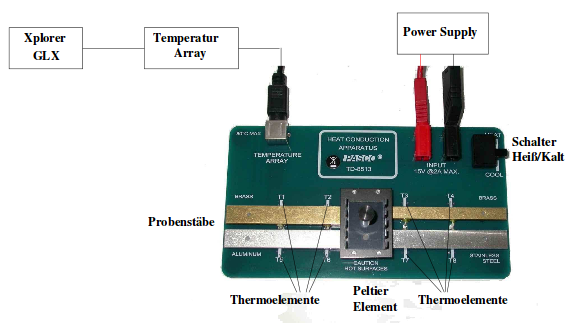
\includegraphics[width=\textwidth ]{Diagramme/v204aufbau.png}
\caption{Skizze zum Versuchsaufbau}
\label{aufbau}
\end{figure}
Zur Messung der Temparaturen der Metallstäbe ist ein Versuchsaufbau auf einer Grundplatte befestigt. Auf dieser Grundplatte sind vier Metallstäbe angebracht, an denen je zwei Thermoelemente in einem festgelegten Abstand befestigt sind. Ein Peltier-Element kann über seine Unterseite das eine Ende der Metallstäbe simultan erhitzen oder kühlen. Über ein Labornetzteil wird das Peltierelement mit Spannung versorgt, durch die Möglichkeit einer Umpolung kann das Peltier-Element entweder kühlen oder heizen. Die Temparaturen an den acht Thermoelementen werden von einem sogenannten Temparaturarray ausgelesen und per Datenkabel an einen Xplorer GLX \footnote{Kleincomputer zur Datenerfassung und Auswertung mit Druckfunktion für Tabellen und Graphen} gesendet.
In Absprache mit der Versuchsleitung wird zum Heizen der Metallstäbe eine Spannung von 8V angelegt und zur Kühlung eine Spannung von 5V. Aufgrund der geringen Effizienz des Peltierelementes würde dieses beim Kühlen warm werden und so die Kühlwirkung verschlechtern.
\subsection{Eigenschaften der Metallstäbe}
Über die vier Metallstäbe sind viele Eigenschaften bekannt. Sie werden in der folgenden Tabelle dargestellt:
\begin{table}[h]
\centering
\begin{tabular}{|c|c|c|c|c|}
\hline
Stoff & Abmessungen [cm] & $\rho \left[ \frac{kg}{m^3} \right] $ & $c \left[ \frac{J}{Kg \cdot K} \right]$ & $ \kappa_{Literatur}$ \\
\hline
Messing (schmal) & 9*0.7*0.4 & 8520 & 385 & 81...105\\
Messing (breit) & 9*1.2*0.4 & 8520 & 385 & 81...105\\
Aluminium  & 9*1.2*0.4 & 2800 & 830 & 200\\
Edelstahl &9*1.2*0.4 & 8000 & 400 & 21\\
\hline
\end{tabular}
\caption{Eigenschaften der Metallstäbe}
\end{table}
\subsection{Statische Methode}
In diesem Versuchsteil soll die Wärmeleitfähigkeit der verschiedenen Metalle ermittelt werden. Dazu werden die Metallstäbe dauerhaft erwärmt, bis der Edelstahl an Messpunkt T7 eine Temparatur von $45^\circ C$ besitzt. Alle fünf Sekunden werden die Temparaturen gemessen und in Abhändigkeit von der Zeit gespeichert. Zur Bestimmung des Metalles mit der besten Wärmeleitung werden die erreichten Temparaturen nach 700 Sekunden notiert. Nach erfolgreicher Messung werden die Metalstäbe aktiv gekühlt, bis sie eine Temparatur erreichen, die unter $30^\circ C$ liegt.
\subsection{Dynamische Methode}
Die dynamische Methode beruht auf dem Angström-Messverfahren. Bei diesem Messverfahren werden die Metallstäbe periodisch erwärmt und gekühlt. Dadurch bildet sich eine Temparaturwelle, die sich durch den Metallstab ausbreitet.
In den dynamischen Messungen werden die Temparaturen alle zwei Sekunden erfasst.
Es werden zwei Messreihen durchgeführt, die sich durch verschiedene Periodendauern unterscheiden. Es wird eine Messung mit einer Periodendauer von 80 Sekunden und eine Messung mit einer Periodendauer von 200 Sekunden durchgeführt. Zwischen den beiden Messreihen werden die Metallstäbe ausreichend gekühlt.

\section{Auswertung}
\subsection{Statische Methode}

Bei der ersten Messung wurden die Stäbe mit dem Peltierelement (Spannung $5V$) erhitzt und die Temperaturen an fernen Thermoelementen ($T_1, T_4, T_5, T_8$) gemessen.Die Abbildungen \ref{T1T4} und \ref{T5T8} zeigen diese Temperaturverläufe graphisch. Desweiteren ist zu erkennen, das die Temperaturen nach $700s$ folgende Werte habe.

\begin{tabular}{@{$\bullet$  }ll}
Messing &$T_1= 42.85 ^\circ C$\\
Messing &$T_4 =  40.69 ^\circ C$\\
Aluminum &$T_5 = 44.92 ^\circ C$\\
Edelstahl &$T_8 =33.17 ^\circ C$\\

\end{tabular}\\
Dieses Ergebnis zeigt qualitativ, dass Aluminum unter den untersuchten Materialien die höchste Wärmeleitfähigkeit besitzt.
\begin{figure}[H]
\centering
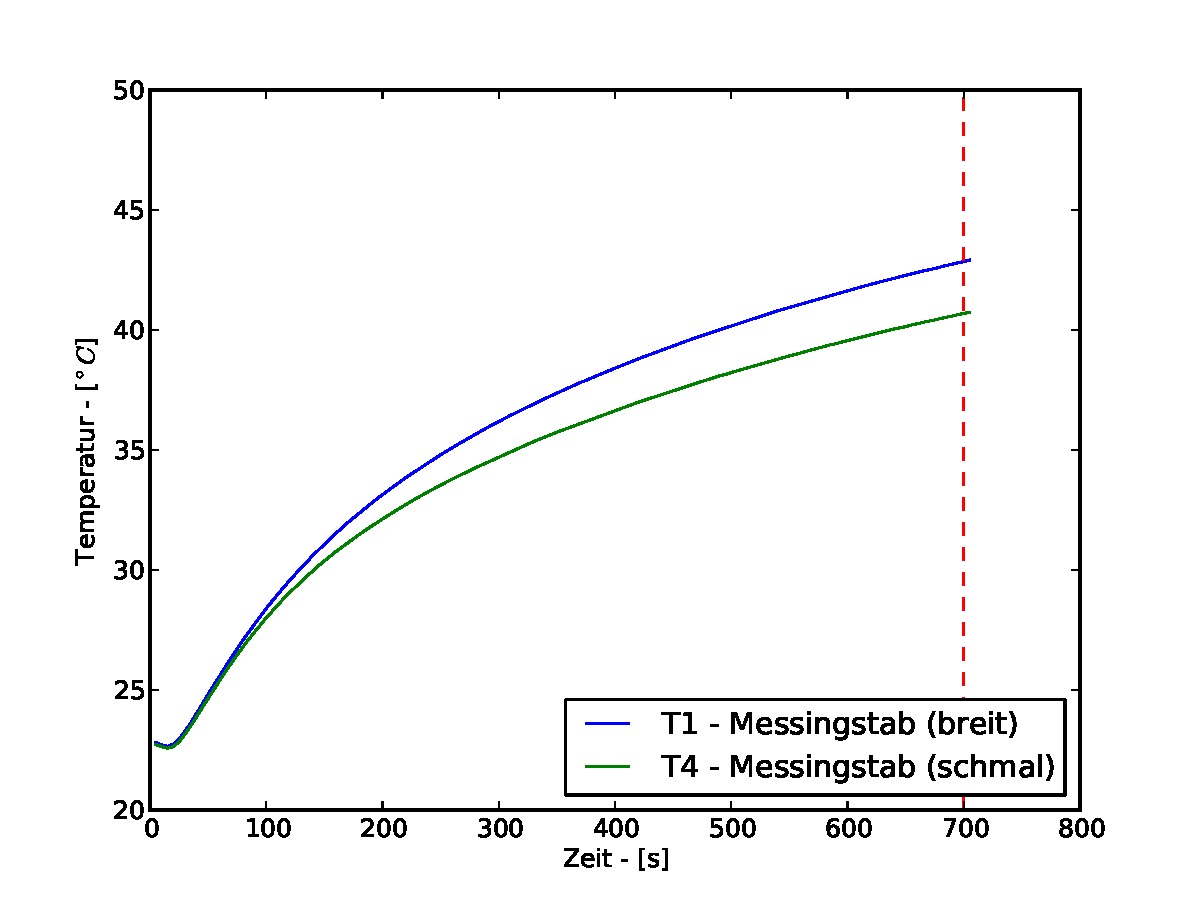
\includegraphics[width = \textwidth]{Diagramme/Abb1.pdf}
\caption{Temperaturverlauf Messing}
\label{T1T4}
\end{figure}
Abbildung 2 zeigt die Temperaturverläufe der beiden Messingstäbe. Die beiden Graphen unterscheiden sich in der Form zunächst recht wenig. Bei $t_0$=0 haben sie eine identische Temperatur. Auch ist die Steigung der beide Graphen zu einem identischen, frühen Zeitpunkt der Erhitzung am größten. Danach nimmt sie kontinuierlich ab. Beide Graphen scheinen zu konvergieren.\newline
Die Graphen unterscheiden sich lediglich im Zahlenwert der Steigung. So hat der breite Messingstab eine leicht höhere Steigung. Aus dieser folgt, dass der Graph der Messung des breiten Messingstabs immer höhere Werte hat und sich die Graphen für die gesamte Messung immer weiter voneinander entfernen.
Es lässt sich also aus der Abbildung 2 entnehmen, dass ein breiter Metallstab Wärme besser leitet als ein schmalerer.
\begin{figure}[H]
\centering
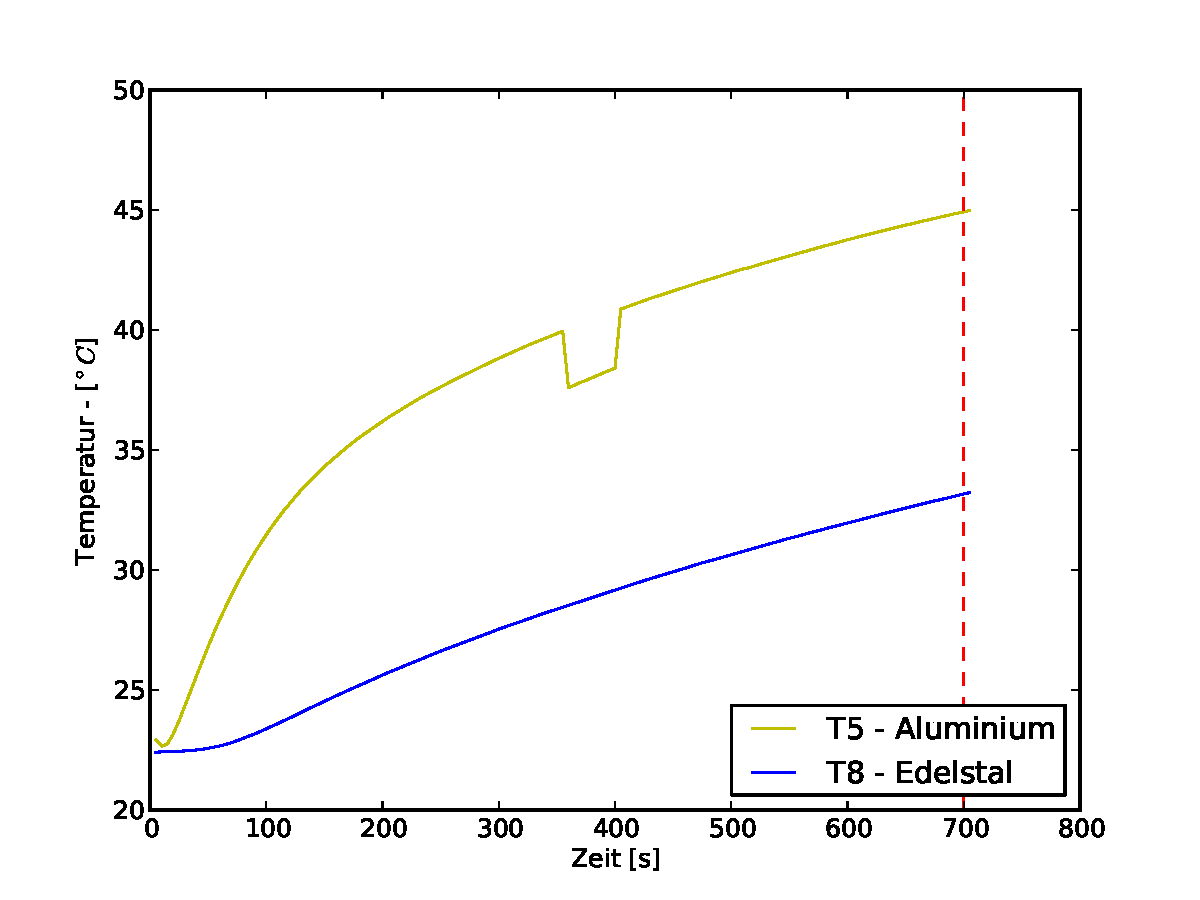
\includegraphics[width = \textwidth]{Diagramme/Abb2.pdf}
\caption{Temperaturverläufe von zwei Messingstäben}
\label{T5T8}
\end{figure}
Die Graphen aus Abbildung 3 weisen deutlichere Unterschiede auf. Der Graph des Aluminiumstabes hat eine deutlich höhere Steigung. Auch erreicht die Steigung beim Aluminiumstab schnell ihr Maximum. Insgesamt erinnert der Graph des Aluminiums an die Graphen des Messings. Der Edelstahlstab hingegen scheint die Wärme viel schlechter zu leiten. Auch sein Graph scheint zu konvergieren, allerdings erreicht der Graph seinen Wendepunkt deutlich später als bei den anderen Metallen.

\subsection{Dynamische Methode}
Bei der ersten Dynamischen wurden die zu untersuchenden St\"abe mit einer Periodendauer von 80 (bzw. 200)  Sekunden abwechselnd gek\"uhlt und erhitzt. Die Abbildungen \ref{dyn_messing}, \ref{dyn_alu} und \ref{dyn_stahl} zeigen jeweils den Temperaturverlauf an zwei 3.0$cm$ voneinander entfernten Messstellen. Im Folgenden werden f\"ur die einzelnen Materialien die Ausbreitungsgeschwindigkeit und die Wellenl\"ange der Temperaturwelle und die W\"armeleitf\"ahigkeit nach der Angstr\"om-Methode berechnet.

\begin{figure}[P]
\centering
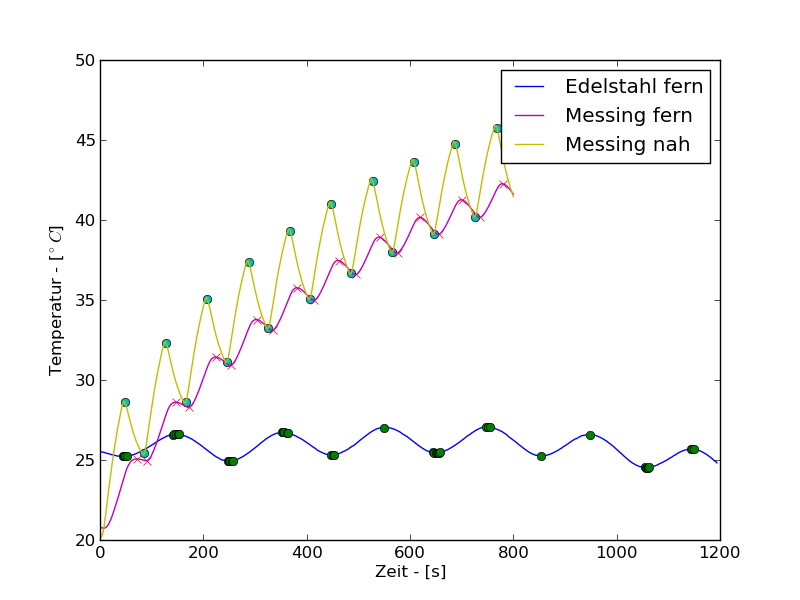
\includegraphics[width=\textwidth]{Diagramme/dyn_messing.png}
\caption{Dynamische Messung Messing}
\label{dyn_messing}
\end{figure}
\begin{figure}[P]
\centering
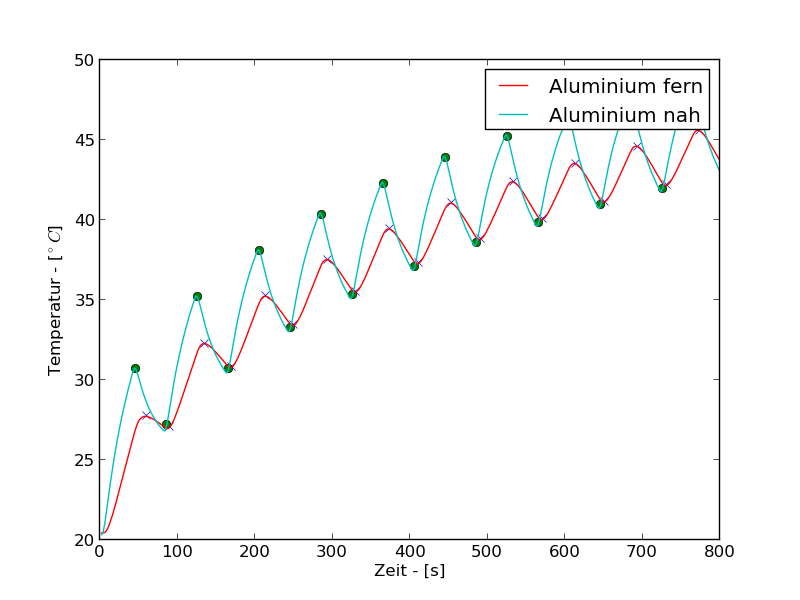
\includegraphics[width=\textwidth]{Diagramme/dyn_alu.png}
\caption{Dynamische Messung Aluminium}
\label{dyn_alu}
\end{figure}
\begin{figure}[P]
\centering
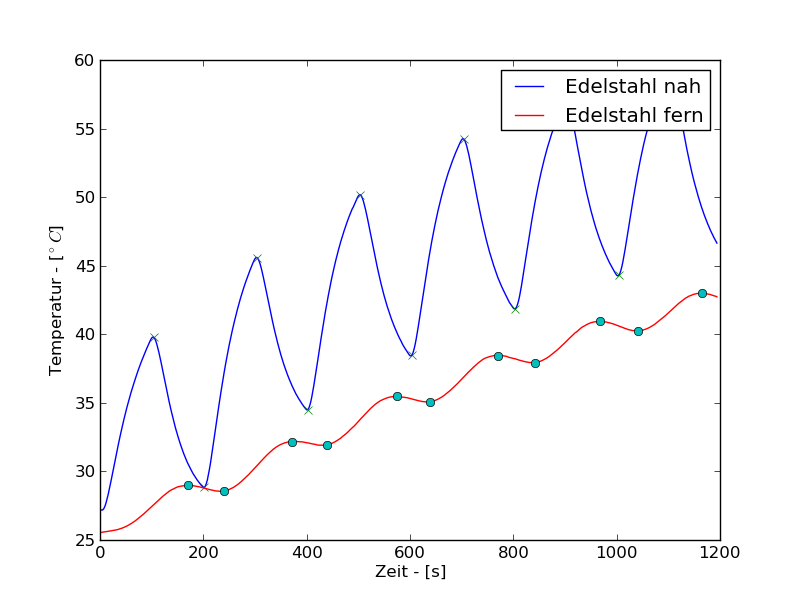
\includegraphics[width=\textwidth]{Diagramme/dyn_stahl.png}
\caption{Dynamische Messung Stahl}
\label{dyn_stahl}
\end{figure}\noindent
Die Wellenl\"ange $\lambda$ einer Welle ist durch
\begin{equation}
\label{wl}
\lambda = \frac{v}{f} = v\cdot T^* = \frac{\Delta x\cdot  T^* }{\Delta t}
\end{equation}
gegeben. Dabei ist $\Delta x$ der Abstand der beiden Messpunkte, $T^*$ die Periodendauer und $\Delta t$ der Phasendifferenz der Welle. Zur Bestimmung von $\Delta t$ wurden ein den Abbilungen die (lokalen) Extrema des Temperaturverlaufsgekennzeichnet. Desweiteren sind diese Punkte in den Tabellen \ref{messing_extr}, \ref{alu_extr} und \ref{stahl_extr} finden.
\begin{table}[P]
\centering
\label{messing_extr}
\begin{tabular}{c|c||c|c}
\multicolumn{2}{c||}{Nah} & \multicolumn{2}{c}{Fern}\\
$t[s]$ & $T[^\circ C]$ & $t[s]$ & $T[^\circ C]$ \\
\hline
72.0 & 25.06 & 128.0 & 32.29\\
90.0 & 24.96 & 166.0 & 28.61\\
148.0 & 28.61 & 208.0 & 35.05\\
172.0 & 28.29 & 246.0 & 31.14\\
224.0 & 31.43 & 288.0 & 37.35\\
254.0 & 30.94 & 326.0 & 33.26\\
304.0 & 33.78 & 368.0 & 39.33\\
334.0 & 33.12 & 406.0 & 35.07\\
382.0 & 35.76 & 448.0 & 41.00\\
414.0 & 34.98s & 486.0 & 36.66\\
462.0 & 37.46 & 528.0 & 42.42\\
496.0 & 36.60 & 566.0 & 37.98\\
542.0 & 38.92 & 608.0 & 43.62\\
576.0 & 37.95 & 646.0 & 39.13\\
620.0 & 40.16 & 688.0 & 44.78\\
656.0 & 39.11 & 726.0 & 40.2\\

\end{tabular}
\caption{Extremwerte der Temperaturwelle in Messing}
\end{table}

\begin{table}[P]
\centering
\label{alu_extr}
\begin{tabular}{c|c||c|c}
\multicolumn{2}{c||}{Nah} & \multicolumn{2}{c}{Fern}\\
$t[s]$ & $T[^\circ C]$ & $t[s]$ & $T[^\circ C]$ \\
\hline
46.0 & 30.7 & 60.0 & 27.72\\
86.0 & 27.16 & 90.0 & 27.05\\
126.0 & 35.17 & 136.0 & 32.27\\
166.0 & 30.7 & 170.0 & 30.8\\
206.0 & 38.04 & 214.0 & 35.23\\
246.0 & 33.26 & 250.0 & 33.41\\
286.0 & 40.33 & 294.0 & 37.52\\
326.0 & 35.31 & 330.0 & 35.49\\
366.0 & 42.24 & 374.0 & 39.43\\
406.0 & 37.06 & 412.0 & 37.32\\
446.0 & 43.85 & 454.0 & 41.04\\
486.0 & 38.58 & 492.0 & 38.82\\
526.0 & 45.18 & 534.0 & 42.38\\
566.0 & 39.82 & 572.0 & 40.05\\
606.0 & 46.3 & 614.0 & 43.51\\
646.0 & 40.92 & 652.0 & 41.15\\
686.0 & 47.45 & 694.0 & 44.59\\
726.0 & 41.96 & 732.0 & 42.19\\
766.0 & 48.4 & 774.0 & 45.57\\

\end{tabular}
\caption{Extremwerte der Temperaturwelle in Aluminium}
\end{table}

\begin{table}[P]
\centering
\label{stahl_extr}
\begin{tabular}{c|c||c|c}
\multicolumn{2}{c||}{Nah} & \multicolumn{2}{c}{Fern}\\
$t[s]$ & $T[^\circ C]$ & $t[s]$ & $T[^\circ C]$ \\
\hline
104.0 & 39.78 & 170.0 & 28.98\\
202.0 & 28.84 & 240.0 & 28.58\\
304.0 & 45.59 & 372.0 & 32.18\\
402.0 & 34.5 & 440.0 & 31.95\\
504.0 & 50.17 & 574.0 & 35.47\\
604.0 & 38.49 & 638.0 & 35.08\\
704.0 & 54.25 & 770.0 & 38.44\\
804.0 & 41.87 & 842.0 & 37.94\\
904.0 & 56.95 & 968.0 & 40.94\\
1004.0 & 44.29 & 1042.0 & 40.25\\
1104.0 & 59.01 & 1166.0 & 42.98\\
\end{tabular}
\caption{Extremwerte der Temperaturwelle in Edelstahl}
\end{table}
 $\Delta t$ ist nun die Zeit zum Beispiel ein Maximum benötigt, um einer Thermosonde zur Anderen zu gelangen, also
\begin{equation}
\Delta t = t_{Fern} - t_{Nah}
\end{equation}
Zur genauerenbestimmung dieser Größe wird der Mittelwert über mehrere Perioden 
\begin{equation}
\overline{\Delta t} = \frac1N \sum^N (t_{Fern}-t_{Nah})
\end{equation}
berechnet. Für die verschiedenen Metalle ergiben sich die fogenden Werte:
\begin{itemize}
\item$\Delta t_{Messing} (12.0\pm1.1)s$
\item $\Delta t_{Aluminium} = (7.1\pm-0.6)s$
\item $\Delta t_{Edelstahl} =  (53\pm5)s$
\end{itemize}
Die ersten beiden Metalle wurden mit einer Periodendauer $T^*$ von $80s$ angeregt und der Edelstahlstab mit einer Periodendauer von $200s$ und die Thermoelemente sind $\Delta x = 0.03m$ vondeinander entfernt. \\Mit Formel (\ref{wl}) können nun die Wellenlängen der einzelnen Temperaturwellen berechnet werden. 
\begin{itemize}
\item $\lambda_{Messing}=(0.200\pm0.018)m$
\item $\lambda_{Aluminium}=(0.340\pm0.027)m$
\item $\lambda_{Edelstahl}=(0.113\pm0.010)m$
\end{itemize}
Zur Berechnung der Temperaturleitfähikeit nach der Angströmmethode wird noch das Amplitudenverhältnis $\frac{A_{Nah}}{A_{Fern}}$ benötigt. Die Amplitude einer Welle entspricht der Hälfte der Differenz der Temperatur zwischem einem Wellenberg ($T_{Max}$) und einem Benachbarten Wellental ($T_{Min}$):
\begin{equation}
A = \frac12\cdot(T_{Max}-T_{Min})
\end{equation}
Analog zu oben wird der Mittelwert
\begin{equation}
\bar {A} = \frac1{2N} \sum^N (T_{Max}-T_{Min})
\end{equation}
über mehrere Perioden gebildet. Mit den Werten aus den Tabellen \ref{messing_extr}, \ref{alu_extr} und \ref{stahl_extr} ergeben sich für die Amplituden:
\begin{table}[H]
\centering
\begin{tabular}{c|l|l}
	& $A_{Nah}[^\circ C]$ & $A_{Fern}[^\circ C]$\\
	\hline
	Messing&$2.85\pm0.34 $& $0.83\pm0.13$ \\
	Aluminium & $3.27\pm0.34$ & $1.46\pm0.14$\\
	Edelstahl & $ 5.2\pm1.3 $ &   $0.92\pm0.24 $\\
\end{tabular}
\end{table}\noindent
\begin{table}[H]

\end{table}\noindent
Mit Gleichung (\ref{kappa}) können dann folgende Werte für die Temperaturleitfähigkeit von Messing, Aluminium und Messing errechnet werden. df
\begin{itemize}
\item $\kappa_{Messing} = (100\pm9)\frac{W}{m K}$
\item $\kappa_{Aluminium} = (184\pm15)\frac{W}{m K}$
\item $\kappa_{Edelstahl} = (15.7\pm-1.4)\frac{W}{m K}$
\end{itemize}
Dieses Ergebnis bestätigt die Beobachtungen bei der statischen Messung und zeigt das Aluminum unter den untersuchten Metallen die höchste Wärmeleitfähigkeit hat.

\section{Diskussion}
Hier kommt die Diskussion hin.
\section{Literatur- und Abbildungsverzeichnis}
Hier befindet sich das Literatur- und Abbildungsverzeichnis.
\section{Anhang}
Hier stehen die im Anhang angefügten Dokumente.
\end{document}
